      
               
                \begin{ledgroupsized}[r]{120mm}
                \footnotesize 
                \pstart                
                \noindent\textbf{\"{U}berlieferung:}   
                \pend
                \end{ledgroupsized}
            
              
                            \begin{ledgroupsized}[r]{114mm}
                            \footnotesize 
                            \pstart \parindent -6mm
                            \makebox[6mm][l]{\textit{L}}Konzept: LH XXXV 15, 6 Bl. 54\textendash 55, Bl. 53, 63. 2 Einzelbl\"{a}tter 4\textsuperscript{o}, 1 Bog. 2\textsuperscript{o} Bl. 53, 63. 3~S. zweispaltig. Textfolge: Bl. 54 r\textsuperscript{o}, Bl. 55 r\textsuperscript{o}, Bl. 63 v\textsuperscript{o}. Bl. 54 oben etwa 5 cm abgetrennt. In der Mitte der rechten Spalte der Vorderseite die Zeichnung \textit{[Fig.~1]}. R\"{u}ckseite leer. Bl. 55 unten etwa 4 cm abgetrennt, R\"{u}ckseite leer. Bl. 63 r\textsuperscript{o} und Bl. 53 ebenfalls leer. Auf allen Seiten rechts Korrekturen und Erg\"{a}nzungen.\\KK 1, Nr. 193 F, G, H \pend
                            \end{ledgroupsized}
                %\normalsize
                \vspace*{5mm}
                \begin{ledgroup}
                \footnotesize 
                \pstart
            \noindent\footnotesize{\textbf{Datierungsgr\"{u}nde}: Leibniz bezieht sich in diesem St\"{u}ck auf die in N. 2\protect\raisebox{-0.5ex}{\tiny{2}} beschriebene Maschine und zeigt, wie sich mit ihrer Hilfe auf See navigieren l\"{a}sst. Das vorliegende St\"{u}ck muss also sp\"{a}ter, d. h. nach 1668/1669 entstanden sein. Da das Wasserzeichen auf Bl. 53 f\"{u}r das Jahr 1669 nachgewiesen ist, gehen wir von der Entstehung des Textes in diesem Jahr aus.}
                \pend
                \end{ledgroup}
            
                \vspace*{8mm}
                \pstart 
                \normalsize
            [54 r\textsuperscript{o}] Longitudines\protect\index{Sachverzeichnis}{longitudo} non per se, sed ut locum in quo sumus, praecise nosse liceat, tanto studio quaeruntur. Id ego jam aliquot ab hinc annis ita consequi posse mihi visus sum. Si quis habeatur index facti itineris tam exactus, ut omnes prorsus tum flexus seu angulos, tum quantitates linearum decursarum ostendat. Qui hactenus de ea re cogitavere, flexus neglexere: ad longitudines\protect\index{Sachverzeichnis}{longitudo} certe applicuit nemo. Ut longitudinem\protect\index{Sachverzeichnis}{longitudo} lineae decursae habeamus, rota\protect\index{Sachverzeichnis}{rota} quadam opus est, quae toties convertitur, quoties linea decursa circumferentiam ejus continet. Hoc fiet si rota\protect\index{Sachverzeichnis}{rota} illa in medium illud perpetuo impingat, in quo fit cursus. Ita rota\protect\index{Sachverzeichnis}{rota} \edtext{renitenti}{\lemma{}\Afootnote{renitenti \textit{ erg.} \textit{ L}}} terrae \edtext{impacta}{\lemma{}\Afootnote{impacta \textit{ erg.} \textit{ L}}} progressu currus\edtext{. Rota citata in navi progressu navis contra renitentem aquam; alia in curru pariter et navi progressu eorum contra retinentem aerem circumagetur.}{\lemma{currus}\Afootnote{ \textit{ (1) }\ , circumagitur \textit{ (2) }\ . Rota [...] aquam \textit{(a)}\ circumagetur \textit{(b)}\ ; alia [...] circumagetur. \textit{ L}}} Sed haec postrema oportet, ut sit subtilior. Ut autem motus aquae aut aeris irregulares nihil turbent, aqua vel aer vix angustis canalibus intrare, et exire debent, in quibus externi motus non sentiantur. Et ut rota\protect\index{Sachverzeichnis}{rota} index non circumagatur quiescente navi\protect\index{Sachverzeichnis}{navis} aut vehiculo, potest firmatus esse eo tempore aditus, aperiendus non nisi cum movetur vehiculum, \edtext{quod}{\lemma{vehiculum,}\Afootnote{ \textit{ (1) }\ ut \textit{ (2) }\ quod \textit{ L}}} sic signabitur, cum duae aliae rotae\protect\index{Sachverzeichnis}{rota} feruntur motu conspirante, alia a vento, seu aere alia ab aqua, vel utraque ab eodem sed diverso situ, ac proinde non congrue, nisi cum movetur ipsa navis\protect\index{Sachverzeichnis}{navis} aut vehiculum. Numerus autem conversionum signabitur eo instrumenti genere, quo constat passus numerari, in denarias rotas\protect\index{Sachverzeichnis}{rota} distributo. Ut flexiones notentur, id sic fiet, si quid sit in navi\protect\index{Sachverzeichnis}{navis}, quod flexis caeteris\hfill solum non\pend
              \begin{center}
              \protect\vspace{5mm}
              %\begin{wrapfigure}{l}{0.6\textwidth}                    
              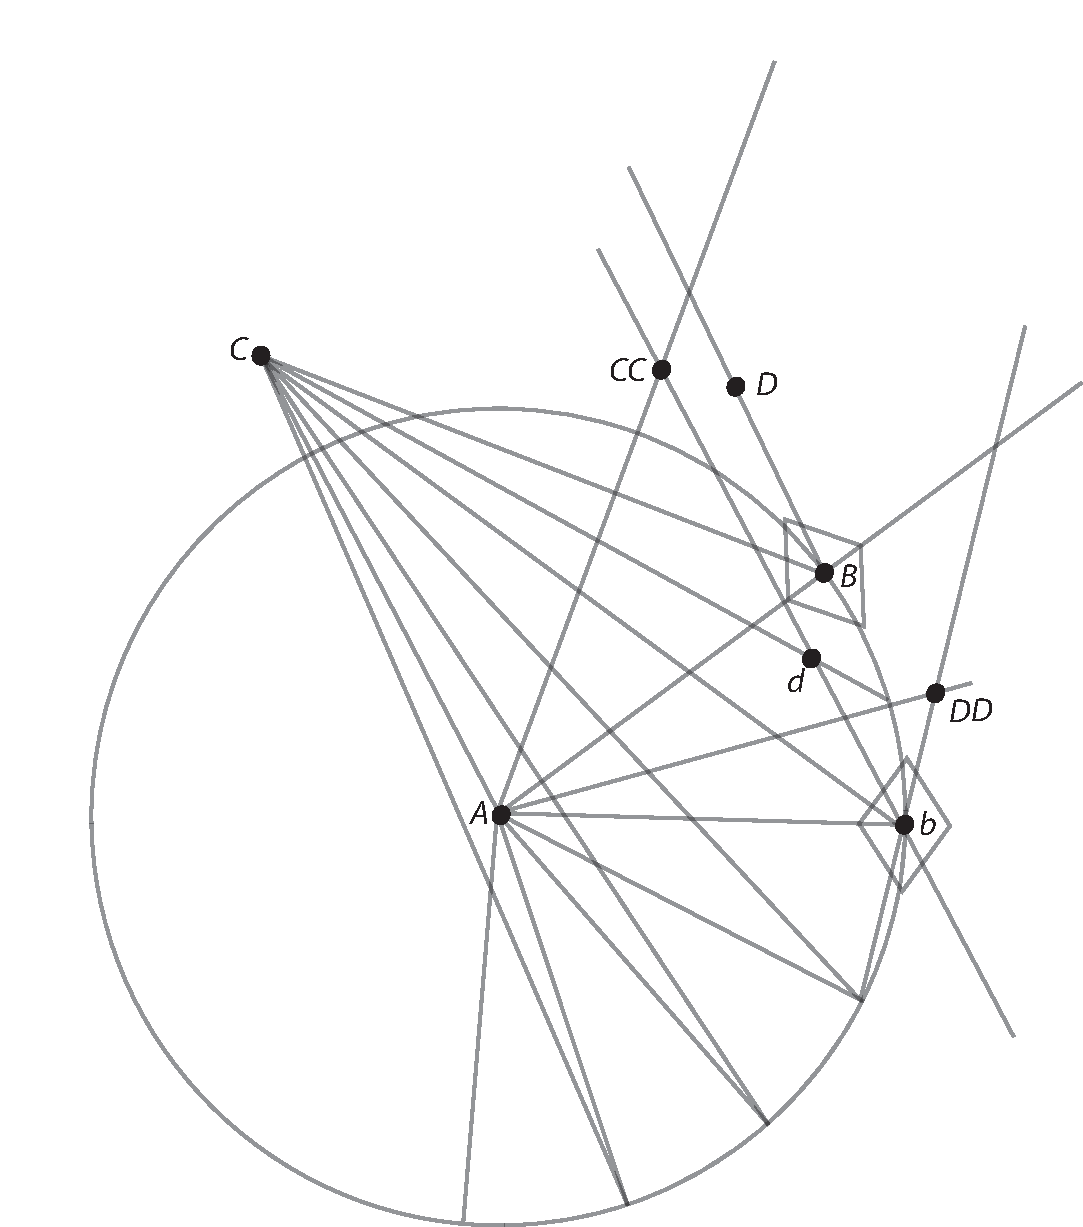
\includegraphics[width=0.8\textwidth]{images/35_15_06_55r}
             \\ \protect\vspace{5mm} \textit{[Fig. 1, tlw. Blindzeichnung]}
              %\protect\vspace{5mm}
              \end{center}
              %\end{wrapfigure}
     \pstart\noindent flectatur. Fit autem flexio in instanti. Eo ergo momento quo caetera omnia \edtext{quae flectuntur}{\lemma{quae}\Afootnote{ \textit{ (1) }\ ad \textit{ (2) }\ flectuntur \textit{ L}}}, reperiendum est, quod non flectatur: tale quid praebet nobis magnes \protect\index{Sachverzeichnis}{magnes} acusve magnetica\protect\index{Sachverzeichnis}{acus!magnetica}. Quae etsi varie declinet a polo\protect\index{Sachverzeichnis}{polus}, constat tamen eo momento quo fit flexio ad certum aliquod punctum respicere; et proinde caeteris flexis inflexum manere. 